\documentclass[11pt,twocolumn]{article}

\usepackage{times}
\usepackage[letterpaper,hmargin=1in,vmargin=1.25in]{geometry}
\usepackage{subfigure}
\usepackage{float}
\usepackage[rflt]{floatflt}
\usepackage{xspace}
\usepackage{cite,alltt}
\usepackage{amsmath,amscd,amssymb}
\usepackage[pdftex]{graphicx}
\usepackage{array}
\usepackage{mathptmx}

\usepackage{vistrails}
\newcommand{\etc}{\emph{etc.}\xspace}
\newcommand{\eg}{\emph{e.g.,}\xspace}
\newcommand{\ie}{\emph{i.e.,}\xspace}


\begin{document}

\title{%Provenance for Visualizations: Beyond Reproduciblity\\
Provenance for Visualizations: Reproducibility and Beyond}
\author{Cl\'audio T. Silva \and Juliana Freire \and Steven P. Callahan}

\maketitle

\begin{abstract}
  The demand for the construction of complex visualizations is growing
  in many disciplines of science, as users are faced with ever
  increasing volumes of data to analyze. The authors present
  VisTrails, an open-source provenance management system that provides
  infrastructure for data exploration and visualization.
\end{abstract}

\section{Introduction}
Computing has been an enormous accelerator for science, leading to an
information explosion in many different fields. Future scientific
advances depend on our ability to comprehend the vast amounts of
data currently being produced and acquired. 
%
To analyze and understand this data, though, we must assemble complex
computational processes and generate insightful visualizations, which
often require combining loosely coupled resources, specialized
libraries, and grid and Web services. Such processes could generate
yet more data, adding to the information overflow scientists currently
deal with.  


Today, the scientific community uses ad hoc approaches to
data exploration, but such approaches have serious limitations. In
particular, scientists and engineers must expend substantial effort
managing data (such as scripts that encode computational tasks, raw
data, data products, images, and notes) and recording provenance
information (that is, all the information necessary for reproducing a
certain piece of data or assertion) so that they can answer basic
questions: Who created a data product and when? When was it modified,
and who modified it? What process was used to create the data product?
Were two data products derived from the same raw data? Not only is
this process time-consuming, it’s also error-prone.  

Without provenance, it’s difficult (and sometimes impossible) to
reproduce and share results, solve problems collaboratively, validate
results with different input data, understand the process used to
solve a particular problem, and reuse the knowledge involved in data
analysis. In addition, data products’ longevity becomes
limited—without precise and sufficient information about how the data
product was generated, its value diminishes significantly.  

\begin{figure}[t]
\centering{
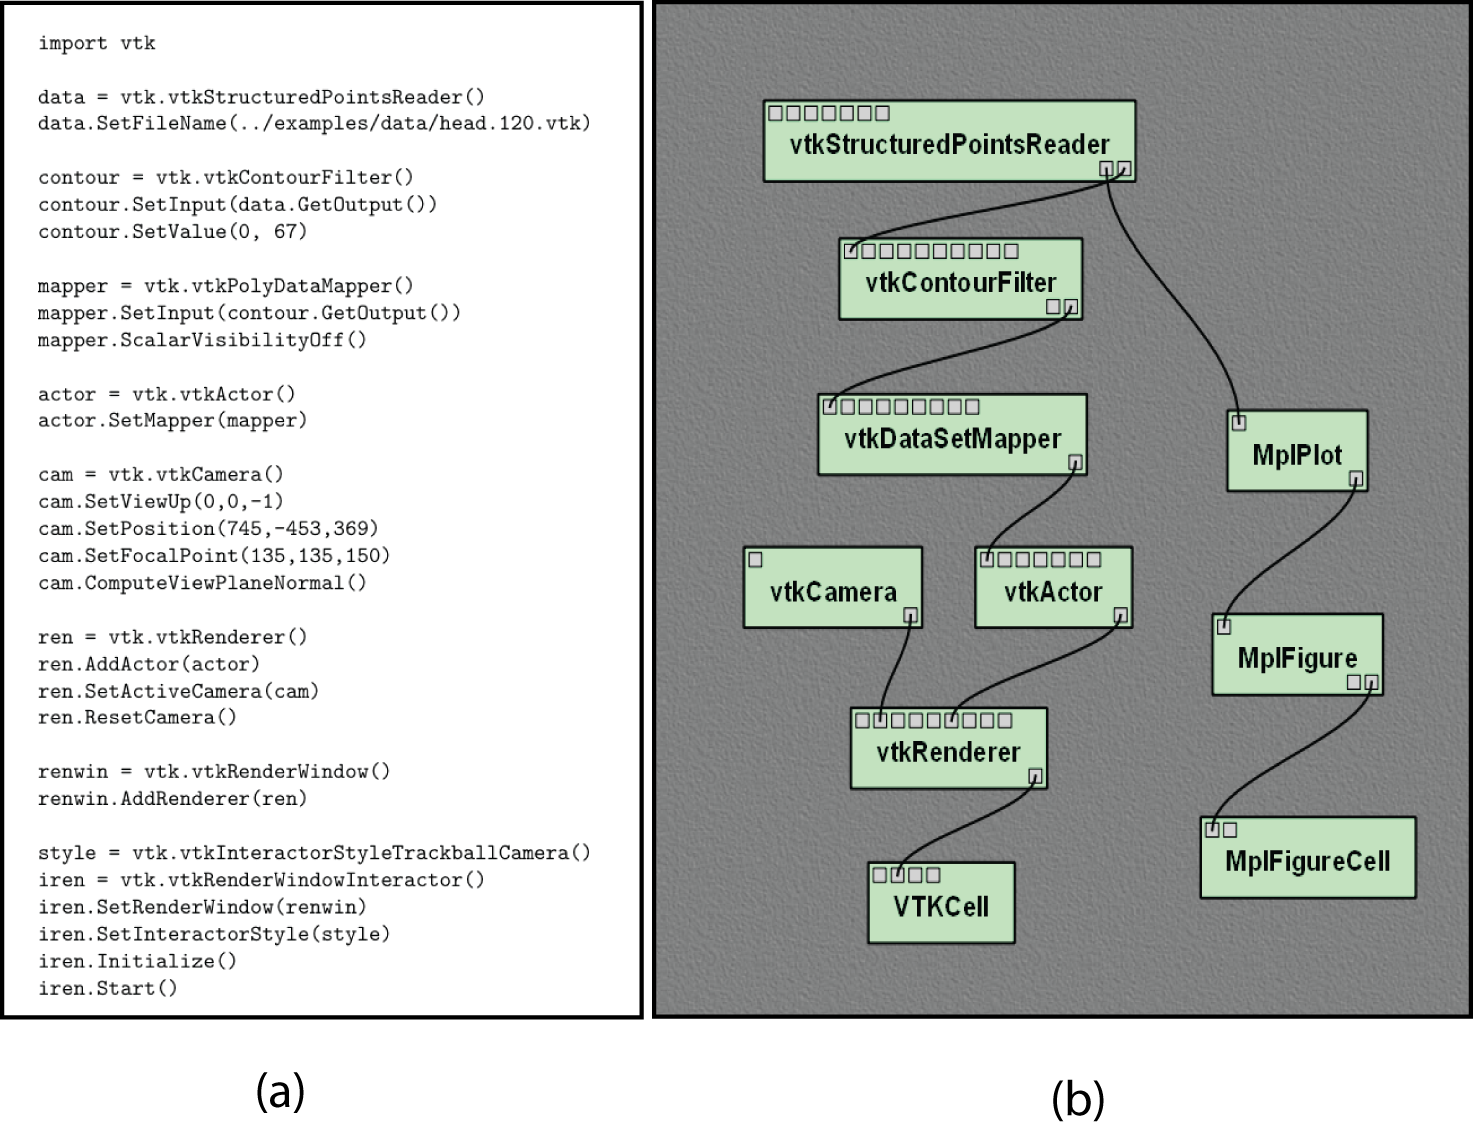
\includegraphics[width=0.9\linewidth, clip=false]{fig1.png}
}
\caption{Dataflow programming for visualization. (a) We commonly use a
  script to describe a pipeline from existing libraries such as the
  Visualization Toolkit (VTK). (b) Visual programming interfaces, such
  as the one VisTrails provides, facilitate the creation and
  maintenance of these dataflow pipelines. The green rectangles
  represent modules, and the black lines represent connections.}
\label{fig:fig1}
\end{figure}

The lack of adequate provenance support in visualization systems
motivated us to build VisTrails, an open source provenance-management
system that provides infrastructure for data exploration and
visualization through workflows. VisTrails transparently records
detailed provenance of exploratory computational tasks and leverages
this information beyond just the ability to reproduce and share
results. In particular, it uses this information to simplify the
process of exploring data through visualization.

\section{Visualization Systems}

Visualization systems such as MayaVi
(\url{http://mayavi.sourceforge.net}) and ParaView
(\url{www.paraview.org})—which are built on top of Kitware's
Visualization Toolkit (VTK)~\cite{Schroeder:2003:VTK}~—as well as
SCIRun (\url{http://software.sci.utah.edu/scirun.html}) enable users
to interactively create and manipulate complex visualizations. Such
systems are based on the notion of data flows~\cite{lee@ieee1995}, and
they provide visual interfaces for producing visualizations by
assembling pipelines out of modules (or functions) connected in a
network. SCIRun supports an interface that lets users directly edit
data flows, giving them complete control. MayaVi and ParaView have a
different interaction paradigm that implicitly builds data flows as
the user makes “task-oriented” choices (such as selecting an
isosurface value).


Although these systems let users create complex visualizations, they
lack the ability to support data exploration at a large scale.
Notably, they don’t adequately support collaborative creation and
exploration of multiple visualizations. Because these systems don’t
distinguish between the definition of a data flow and its instances,
to execute a given data flow with different parameters (for example,
different input files), users must manually set these parameters
through a GUI. Clearly, this process doesn’t scale to more than a few
visualizations at a time. Additionally, modifications to parameters or
to a data flow’s definition are destructive—the systems don’t maintain
any change history. This requires the user to first construct the
visualization and then remember the input data sets, parameter values,
and the exact dataflow configuration that led to a particular image.


Finally, before constructing a visualization, users must often
acquire, generate, or transform a given data set—for example, to
calibrate a simulation, they must obtain data from sensors, generate
data from a simulation, and finally construct and compare the
visualization for both data sets. Most visualization systems, however,
don’t give users adequate support for creating the complex pipelines
that use multiple libraries and services.

\begin{figure*}[t]
\centering{
%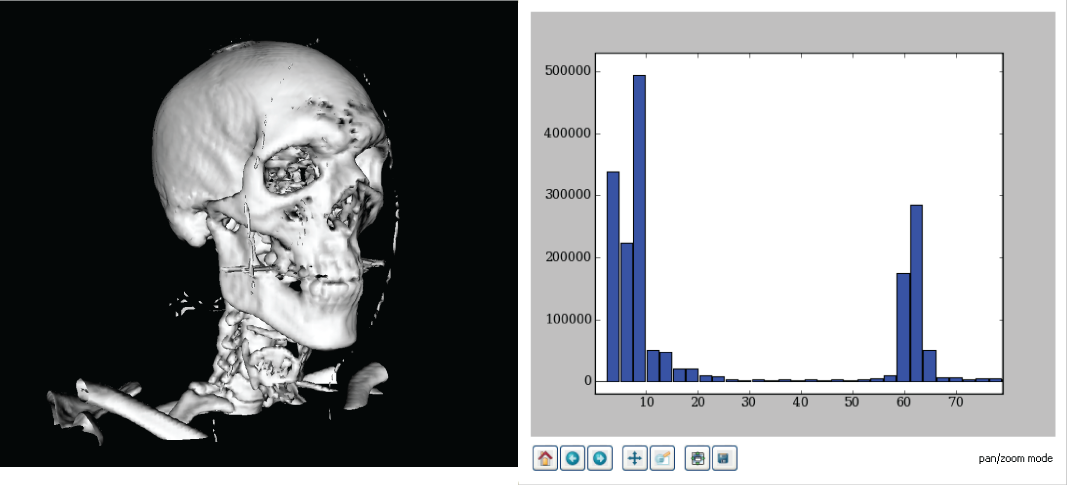
\includegraphics[width=0.9\linewidth, clip=false]{fig2.png}
\vistrail[host=vistrails.org,
db=vistrails,
vtid=4,
version=655,
tag=demo11,
showspreadsheetonly]{width=4cm}
}
\caption{The end result of the script or VisTrails pipeline (see
  Figure~\ref{fig:fig1}) is a set of interactive visualizations.}
\label{fig:histogram}
\end{figure*}

\section{VisTrails: Provenance for Visualization}
VisTrails (\url{www.vistrails.org}) is a new visualization system we
developed at the University of Utah that provides a comprehensive
provenance-management infrastructure and can be easily combined with
existing visualization libraries. Unlike previous systems, VisTrails
uses an action-based provenance model that uniformly captures changes
to both parameter values and pipeline definitions by unobtrusively
tracking all changes that users make to pipelines in an exploration
task. We refer to this detailed provenance of the pipeline evolution
as a visualization trail, or vistrail. 

The stored provenance ensures that users will be able to
reproduce the visualizations and lets them easily navigate through the
space of pipelines created for a given exploration task. The VisTrails
interface lets users query, interact with, and understand the
visualization process’s history. In particular, they can return to
previous versions of a pipeline and change the specification or
parameters to generate a new visualization without losing previous
changes.  

\begin{figure*}[t]
\centering{
%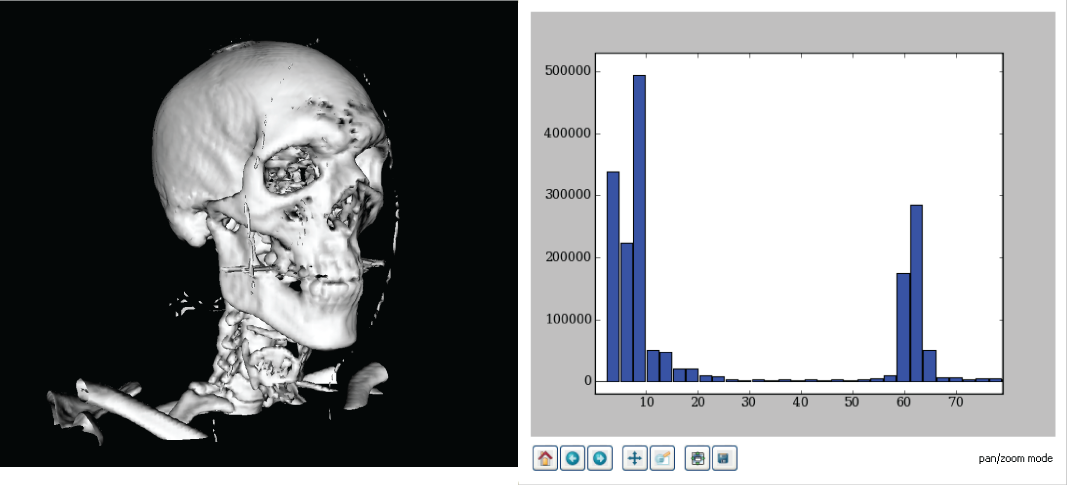
\includegraphics[width=0.9\linewidth, clip=false]{fig2.png}
\vistrail[host=vistrails.org,
db=vistrails,
vtid=4,
version=613,
showspreadsheetonly,
pdf]{width=4cm}
}
\caption{The end result of the script or VisTrails pipeline (see
  Figure~\ref{fig:fig1}) is a set of interactive visualizations.}
\label{fig:histogram_pdf}
\end{figure*}

Another important feature of the action-based provenance model is that
it enables a series of operations that greatly simplify the
exploration process and could reduce the time to insight. In
particular, it allows the flexible reuse of pipelines and provides a
scalable mechanism for creating and comparing numerous visualizations
as well as their corresponding pipelines. Although we originally
built VisTrails to support exploratory visualization tasks, its
extensible infrastructure lets users integrate a wide range
of libraries. This makes the system suitable for other exploratory
tasks, including data mining and integration.  

\section{Creating an Interactive Visualization with VisTrails}
To illustrate the issues involved in creating visualizations and how
provenance can aid in this process, we present the following scenario,
common in medical data visualization.

Starting from a volumetric computed tomography (CT) data set, we
generate different visualizations by exploring the data through volume
rendering, isosurfacing (extracting a contour), and slicing. Note that
with proper modifications, this example also works for visualizing
other types of data (for example, tetrahedral meshes). 

\subsection{Dataflow Processing Networks and Visual Programming}
A useful paradigm for building visualization applications is the
\emph{dataflow model}. A data flow is a directed graph in which nodes
represent computations, and edges represent data streams: each node or
module corresponds to a procedure that’s applied on the input data and
generates some output data as a result. The data flow in the graph
determines the order in which a dataflow system executes the
processing nodes. In visualization, we commonly refer to a dataflow
network as a visualization pipeline. (For this article, we use the
terms workflow, data flow, and pipeline interchangeably.)
Figure~\ref{fig:fig1}b shows an example of the data flow used to
derive the images shown in Figure~\ref{fig:histogram}. The green
rectangles represent modules, and the black lines represent
connections. Most of the modules in Figure~\ref{fig:fig1} are from VTK, and
labels on each module indicate the corresponding VTK class. In this
figure, we naturally think of data flowing from top to bottom,
eventually being rendered and presented for display.

\bibliography{example2} 
\bibliographystyle{abbrv}
\end{document}